\pagebreak
\thispagestyle{empty}
\movetoevenpage
\begin{figure}
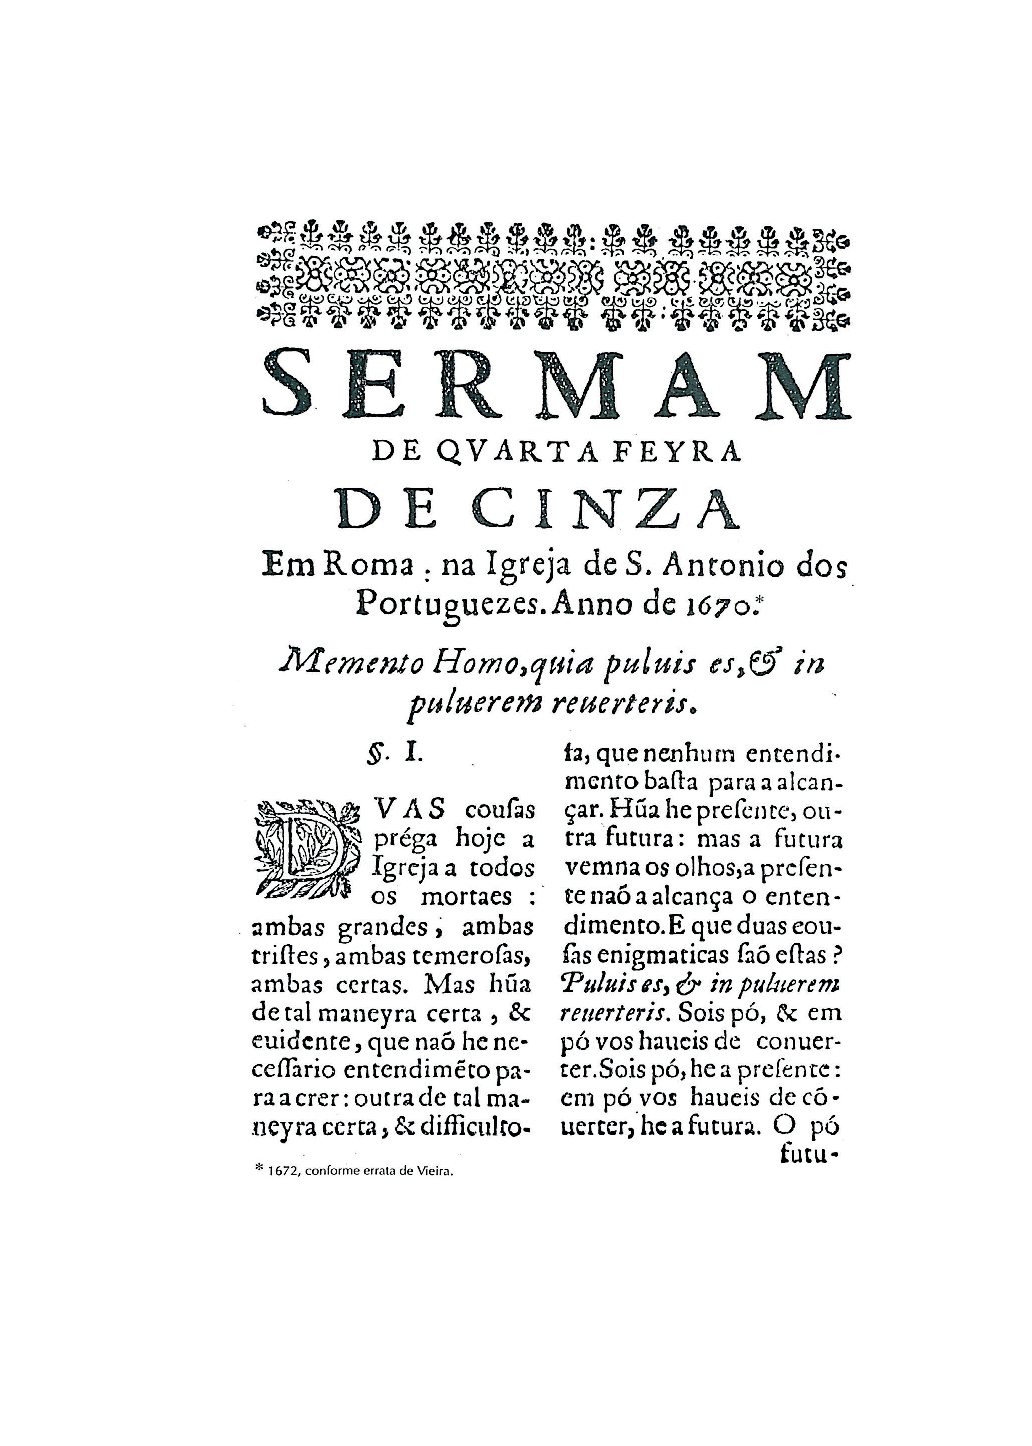
\includegraphics[width=\textwidth]{./imgs/cinza.pdf}  
\end{figure}

\chapter{Sermão de quarta"-feira de cinza}

\begin{quotation}
\noindent{}Em Roma, na Igreja de S.\,Antônio dos Portugueses, ano de 1672
\end{quotation}

\epigraph{\emph{Memento homo, quia pulvis es, et in pulverem reverentis}.}{}

\section{I}

\noindent{}Duas coisas prega hoje a Igreja a todos os mortais, ambas grandes, ambas
tristes, ambas temerosas, ambas certas. Mas uma de tal maneira certa e
evidente, que não é necessário entendimento para crer; outra de tal
maneira certa e dificultosa, que nenhum entendimento basta para a
alcançar. Uma é presente, outra futura, mas a futura vêem"-na os olhos, a
presente não a alcança o entendimento. E que duas coisas enigmáticas são
estas? \emph{Pulvis es, tu in pulverem reverteris:} Sois pó, e em pó vos
haveis de converter. Sois pó, é a presente; em pó vos haveis de
converter, é a futura. O pó futuro, o pó em que nos havemos de
converter, vêem"-no os olhos; o pó presente, o pó que somos, nem os olhos
o vêem, nem o entendimento o alcança. Que me diga a Igreja que hei de
ser pó: \emph{Jn pulverem reverteris}, não é necessário fé nem
entendimento para o crer. Naquelas sepulturas, ou abertas ou cerradas, o
estão vendo os olhos. Que dizem aquelas letras? Que cobrem aquelas
pedras? As letras dizem pó, as pedras cobrem pó, e tudo o que ali há é o
nada que havemos de ser: tudo pó. Vamos, para maior exemplo e maior
horror, a esses sepulcros recentes do Vaticano. Se perguntardes de quem
são pó aquelas cinzas, responder"-vos"-ão os epitáfios, que só as
distinguem: Aquele pó foi Urbano, aquele pó foi Inocêncio,
aquele pó foi Alexandre, e este que ainda não está de todo desfeito, foi
Clemente. De sorte que para eu crer que hei de ser pó, não é necessário
fé, nem entendimento, basta a vista. Mas que me diga e me pregue hoje a
mesma Igreja, regra da fé e da verdade, que não só hei de ser pó de
futuro, senão que já sou pó de presente: \emph{Pulvis es?} Como o pode
alcançar o entendimento, se os olhos estão vendo o contrário? É possível
que estes olhos que vêem, estes ouvidos que ouvem, esta língua que fala,
estas mãos e estes braços que se movem, estes pés que andam e pisam,
tudo isto, já hoje é pó: \emph{Pulvis es?} Argumento à Igreja com a
mesma Igreja: \emph{Memento homo}. A Igreja diz"-me, e supõe que sou
homem: logo não sou pó. O homem é uma substância vivente, sensitiva,
racional. O pó vive? Não. Pois como é pó o vivente? O pó sente? Não.
Pois como é pó o sensitivo? O pó entende e discorre? Não. Pois como é pó
o racional? Enfim, se me concedem que sou homem: \emph{Memento homo},
como me pregam que sou pó: \emph{Quia pulvis es?} Nenhuma coisa nos
podia estar melhor que não ter resposta nem solução esta dúvida. Mas a
resposta e a solução dela será a matéria do nosso discurso. Para que eu
acerte a declarar esta dificultosa verdade, e todos nós saibamos
aproveitar deste tão importante desengano, peçamos àquela Senhora, que
só foi exceção deste pó, se digne de nos alcançar graça. \emph{Ave Maria}.

\section{II}

Enfim, senhores, não só havemos de ser pó, mas já somos pó: \emph{Pulvis
es}. Todos os embargos que se podiam pôr contra esta sentença universal
são os que ouvistes. Porém como ela foi pronunciada definitiva e
declaradamente por Deus ao primeiro homem e a todos seus descendentes,
nem admite interpretação, nem pode ter dúvida. Mas como pode ser? Como
pode ser que eu que o digo, vós que o ouvis, e todos os que vivemos
sejamos já pó: Pulvis es?
A razão é esta. O homem, em qualquer estado que esteja, é certo que foi
pó, e há de tornar a ser pó. Foi pó, e há de tomar a ser pó? Logo é pó.
Porque tudo o que vive nesta vida, não é o que é: é o que foi e o que há
de ser. Ora vede.

No dia aprazado em que Moisés e os magos do Egito haviam de fazer prova
e ostentação de seus poderes diante de eI rei Faraó, Moisés estava só
com Arão de uma parte, e todos os magos da outra. Deu sinal o rei,
mandou Moisés a Arão que lançasse a sua vara em terra, e converteu"-se
subitamente em uma serpente viva e tão temerosa, como aquela de que o
mesmo Moisés no deserto se não dava por seguro. Fizeram todos os magos o
mesmo: começam a saltar e a ferver serpentes, porém a de Moisés investiu
e avançou a todas elas intrépida e senhorilmente, e assim, vivas como
estavam, sem matar nem despedaçar, comeu e engoliu a todas. Refere o
caso a Escritura, e diz estas palavras: \emph{Devoravit virga Aaron
virgas eorum:} a vara de Arão comeu e engoliu as dos egípcios. Aqui reparo.
Parece que não havia de dizer a Vara, senão a Serpente. A vara
não tinha boca para comer, nem dentes para mastigar, nem garganta para
engolir, nem estômago para recolher tanta multidão de serpentes. A
serpente, em que a vara se converteu, sim, porque era um dragão vivo,
voraz e terrível, capaz de tamanha batalha e de tanta façanha. Pois, por
que diz o texto que a vara foi a que fez tudo isto, e não a serpente?
Porque cada um é o que foi e o que há de ser. A vara de Moisés, antes de
ser serpente, foi vara, e depois de ser serpente, tornou a ser vara; a
serpente que foi vara e há de tornar a ser vara não é serpente, é vara:
\emph{Virga Aaron}. E verdade que a serpente naquele tempo estava viva,
e andava, e comia, e batalhava, e vencia, e triunfava, mas como tinha
sido vara, e havia de tornar a ser vara, não era o que era: era o que
fora e o que havia de ser: \emph{Virga}.

Ah! serpentes astutas do mundo, vivas e tão vivas! Não vos fieis
da vossa vida nem da vossa viveza; não sois o que cuidais nem o que
sois: sois o que fostes e o que haveis de ser. Por mais que vós vejais
agora um dragão coroado e vestido de armas douradas, com a couda
levantada e retorcida açoitando os ventos, o peito inchado, as asas
estendidas, o colo encrespado e soberbo, a boca aberta, dentes
agudos, língua trifitricada, olhos cintilantes, garras e unhas
rompentes, por mais que se veja esse dragão já tremular na bandeira dos
lacedemônios, já passear nos jardins das hespérides,já guardar os
tesouros de Midas, ou seja dragão volante entre os meteoros, ou dragão
de estrelas entre as constelações, ou dragão de divindade afetada entre
as hierarquias, se foi vara, e há de ser vara, é vara; se foi terra, e
há de ser terra, é terra; se foi nada, e há de ser nada, é nada, porque
tudo o que vive neste mundo é o que foi e o que há de ser. Só Deus é o
que é, mas por isso mesmo. Por isso mesmo. Notai.

Apareceu Deus ao mesmo Moisés nos desertos de Midiã; manda"-o que leve a nova da liberdade ao povo cativo, e perguntando
Moisés quem havia de dizer que o mandava, para que lhe dessem crédito,
respondeu Deus e definiu"-se: \emph{Ego sum qui sum:} Eu sou o que sou. %(Êx. 3,14)
Dirás que o que é te manda: \emph{Qui est misit me ad vos?
Qui est?} O que é? E que nome, ou que distinção é esta? Também Moisés é
o que é, também Faraó é o que é, também o povo, com que há de falar, é o
que é. Pois se este nome e esta definição toca a todos e a tudo, como a
toma Deus só por sua? E se todos são o que são, e cada um é o que é, por
que diz Deus não só como atributo, senão como essência própria da sua
divindade: \emph{Ego sum qui sum:} Eu sou o que sou? Excelentemente S.\,Jerônimo, respondendo com as palavras do Apocalipse: \emph{Qui est, et
qui erat, et qui venturus est}, Sabeis por que diz Deus: \emph{Ego sum
qui sum?} Sabeis por que só Deus é o que é? Porque só Deus é o que foi e
o que há de ser. Deus é Deus, e foi Deus, e há de ser Deus; e só quem é
o que foi e o que há de ser, é o que é: \emph{Qui est, et qui erat, et
qui venturus est. Ego sum qui sum}. De maneira que quem é o que foi e o
que há de ser, é o que é, e este é só Deus. Quem não é o que foi e o que
há de ser, não é o que é: é o que foi e o que há de ser: e esses somos
nós. Olhemos para trás: que é o que fomos? Pó. Olhemos para diante: que
é o que havemos de ser? Pó. Fomos pó e havemos de ser pó? Pois isso é o
que somos: \emph{Pulvis es}.

Eu bem sei que também há deuses da terra, e que esta terra onde
estamos foi a pátria comum de todos os deuses, ou próprios, ou
estrangeiros. Aqueles deuses eram de diversos metais; estes são de
barro, ou cru ou mal cozido, mas deuses. Deuses na grandeza, deuses na
majestade, deuses no poder, deuses na adoração, e
também deuses no nome: \emph{Ego dixi, dii estis}. Mas se houver, que
pode haver, se houver algum destes deuses que cuide ou diga: \emph{Ego
sum qui sum}, olhe primeiro o que foi e o que há de ser. Se foi Deus, e
há de ser Deus, é Deus: eu o creio e o adoro; mas se não foi Deus, nem
há de ser Deus, se foi pó, e há de ser pó, faça mais caso da sua
sepultura que da sua divindade. Assim lho disse e os desenganou o mesmo
Deus que lhes chamau deuses: \emph{Ego dixi, dii estis. Vos outem sicut
homines moremini}. Quem foi pó e há de ser pó, seja o que quiser e
quanto quiser, é pó: \emph{Pulvis es}.

\section{III}

Parece"-me que tenho provado a minha razão e a consequência dela. Se a
quereis ver praticada em próprios termos, sou contente. Praticaram este
desengano dois homens que sabiam mais de nós que nós: Abraão e Jó, com
outro \emph{memento} como o nosso, dizia a Deus: \emph{Memento quaeso,
quod sicuit lutum feceris me, et in pulverem deduces me:} Lembrai"-vos,
Senhor, que me fizestes de pó, e que em pó me haveis de tornar. %(Jó l0, 9)
Abraão, pedindo licença ou atrevimento para falar a Deus:
\emph{Loquar ad Dominum, cum sim pulvis et cinis:} Falar"-vos"-ei, Senhor,
ainda que sou pó e cinza. Já vedes a diferença dos % (Gên. 18, 27)
termos que não pode ser maior, nem também mais natural ao nosso intento.
Jó diz que foi pó e há de ser pó; Abraão não diz que foi, nem que há de
ser, senão que já é pó: \emph{Cum sim pulvis et cinis}. Se um destes
homens fora morto e outro vivo, falavam muito propriamente, porque todo
o vivo pode dizer: Eu fui pó, e hei de ser pó; e um morto, se falar,
havia de dizer: Eu já sou pó. Mas Abraão que disse isto, não estava
morto, senão vivo, como Jó; e Abraão e Jó não eram de diferente metal,
nem de diferente natureza. Pois se ambos eram da mesma natureza, e ambos
estavam vivos, como diz um que já é pó, e outro não diz que o é, senão
que o foi e que o há de ser? Por isso mesmo. Porque Jó foi pó e há de
ser pó, por isso Abraão é pó. Em Jó falou a morte, em
Abraão falou a vida, em ambos a natureza. Um descreveu"-se pelo passado e
pelo futuro, o outro definiu"-se pelo presente; um reconheceu o efeito, o
outro considerou a cousa; um disse o que era, o outro declarou o porquê.
Porque Jó e Abraão e qualquer outro homem foi pó, por isso já é pó.
Fostes pó e haveis de ser pó como Jó? Pois já sois pó como Abraão:
\emph{Cum sim pulvis et cinis}.

Tudo temos no nosso texto, se bem se considera, porque as segundas
palavras dele não só contêm a declaração, senão também a razão das
primeiras. \emph{Pulvis es:} sois pó. E por quê? Porque in
\emph{pulverem mverteris:} porque fostes pó e haveis de tomar a ser pó.
Esta é a força da palavra reverteris, a qual não só significa o po que
havemos de ser; senão também a pó que somos. Por isso não diz:
\emph{convertetis}, converter"-vos"-eis em pó, senão: \emph{reverteris},
tomareis a ser o pó que fostes. Quando dizemos que os mortos se
convertem em pó, falamos impropriamente, porque aquilo não é conversão,
é reversão: \emph{reverteris}. É tornar a ser na morte a pó que somos no
nascimento; é tornar a ser na sepultura a pó que somos no campo
damasceno. E porque somos pó e havemos de tomar a ser pó: Ia
\emph{pulverem neverteris}, por isso já somos pó: \emph{Pulvis es}.
Não é exposição minha, senão formalidade do mesmo texto, com que Deus
pronunciou a sentença de morte contra Adão: \emph{Donec reverteris in
terram de qua sumptus es: quia pulvis es}: Até que tomes % (Gên. 3,19)
a ser a tenra de que fostes formado, porque és pó. De maneira que a
razão e o porquê de sermos pó: \emph{Qutíapulvis es}, é porque somos pó,
e havemos de tomar a ser pó: \emph{Donec revertaris in terram de qua
sumptus es}.

Só parece que se pode opor ou dizer em contrário, que aquele
\emph{donec:} até que, significa tempo em meio entre o pó que somos e o
pó que havemos de ser, e que neste meio tempo não somos pó. Mas a mesma
verdade divina que disse: \emph{donec}, disse também: \emph{pulvis es}.
E a razão desta consequência está no \emph{reverteris}, porque a
reversão com que tornamos a ser a pó que fomos começa circularmente, não
do último senão do primeiro ponto da vida. Notai. Esta nossa chamada
vida não é mais que um círculo que fazemos de pó a pó: do pó que fomos
ao pó que havemos de ser. Uns fazem o círculo maior, outros menor,
outros mais pequeno, outros mínimo: \emph{De utero transíatus ad
tumulum}. Mas, ou a caminho seja largo, ou breve, ou
brevíssimo, como é círculo de pó a pó, sempre e em qualquer parte da
vida somos pó. Quem vai circularmente de um ponto para o mesmo ponto,
quanto mais se aparta dele tanto mais se chega para ele; e quem quanto
mais se aparta mais se chega, não se aparta. O pó que foi nosso
princípio, esse mesmo, e não outro, é o nosso fim, e porque caminhamos
circularmente deste pó para este pó, quanto mais parece que nos
apartamos dele, tanto mais nos chegamos para ele; o passo que nos
aparta, esse mesmo nos chega; o dia que faz a vida, esse mesmo a desfaz.
E como esta roda que anda e desanda juntamente sempre nos vai moendo,
sempre somos pó. Por isso, quando Deus intimau a Adão a reversão ou
revolução deste circulo: \emph{Donec revertaris}, das premissas: pó
foste, e pó serás, tirou por consequência: pó és: Quia pulvis es. Assim
que desde o primeiro instante da vida até o último nos devemos persuadir
e assentar conosco, que não só somos e havemos de ser pó, senão que já a
somos, e por isso mesmo. Foste pó e hás de ser pó? És pó: \emph{Pulvis
es.}

\section{IV}

Ora, suposto que já somos pó, e não pode deixar de ser, pois Deus o
disse, perguntar"-me"-eis e com muita razão, em que nos distinguimos logo
os vivos dos mortos? Os mortos são pó, nós também somos pó: em que nos
distinguimos uns dos outros? Distinguimo"-nos os vivos dos mortos, assim
como se distingue o pó do pó. Os vivos são pó levantado, os mortos são
pó caído: os vivos são pó que anda, os mortos são pó que jaz: \emph{Hic
jacet}. Estão essas praças no verão cobertas de pó; dá um pé"-de"-vento,
levanta"-se o pó no ar, e que faz? O que fazem as vivos, e muitos vivos.
Não aquieta o pó, nem pode estar queda: anda, corre, voa, entrapar esta
rua, sai por aquela; já vai adiante, já torna atrás; tudo enche, tudo
cobre, tudo envolve, tudo perturba, tudo cega, tudo penetra, em tudo e
por tudo se mete, sem aquietar, nem sossegar um momento, enquanto o
vento dura. Acalmau o vento, cai o pó, e onde o vento parou, ali fica,
ou dentro de casa, ou na rua, ou em cima de um telhado, ou no mar; ou no
rio, ou no monte, ou na campanha. Não é assim? Assim é. E que pó, e que
vento é este? O pó somos nós:
\emph{Quia pulvis es}; o vento é a nossa vida: \emph{Quia ventus es vita
mea}. Deu o vento, levantou"-se o pó; parou a vento, caiu. Deu o % (Jó 7,7)
vento, eis o pó levantado: esses são os vivos. Parou o vento, eis o pó
caído: estes são os mortos. Os vivos pó, os mortos pó; os vivos pó
levantado, os mortos pó caído; os vivos pó com vento, e por isso vãos;
os mortos pó sem vento, e por isso sem vaidade. Esta é a distinção, e
não há outra.

Nem cuide alguém que é isto metáfora ou comparação, senão realidade
experimentada e certa. Forma Deus de pó aquela primeira estátua, que
depois se chamau carpa de Adão. Assim o diz o texto original:
\emph{Formavit Deus hominem de pulvere terrae}. A figura era % (Gên. 2,7)
humana e muito primorosamente delineada, mas a substância ou a matéria
não era mais que pó. A cabeça pó, o peito pó, os braços pó, os olhos, a
boca, a língua, o coração, tudo pó. Chega"-se pais Deus à estátua, e que
fez? \emph{Jnspiravit in faciem ejus:} Assoprou"-a. E tanto % (Gên. 2,7)
que o vento do assopro deu no pó: \emph{Et factus est homo in animam
viventem:} eis o pó levantado e vivo; já é homem,já se chama Adão. Ah!
pó, se aquietaras e pararas aí! Mas pó assoprada, e com vento, como
havia de aquietar? Ei"-la abaixa, ei"-lo acima, e tanto acima, e tanto
abaixo, dando uma tão grande volta, e tantas voltas. Já senhor do
universo, já escravo de si mesma; já só, já acompanhado; já nu, já
vestido; já coberta de folhas; já de peles; já tentada, já vencido; já
homiziada, já desterrada; já pecador, já penitente, e para maior
penitência, pai, chorando os filhos, lavrando a terra, recolhendo
espinhos por frutos, suando, trabalhando, lidando, fatigando, com tantos
vaivéns do gosto e da fortuna, sempre em uma roda viva. Assim andou
levantado o pó enquanto durou o vento. O vento durou muito, porque
naquele tempo eram mais largas as vidas, mas alfim parou. E que lhe
sucedeu no mesmo ponto a Adão? O que sucede ao pó. Assim como o vento a
levantou, e o sustinha, tanto que o vento parou, caiu. Pó levantado,
Adão vivo; pó caído, Adão morto: \emph{Et mortus est.}

Este foi o primeiro pó, e o primeiro vivo, e o primeiro condenado
à morte, e esta é a diferença que há de vivos a mortos, e de pó a pó.
Por isso na Escritura o morrer se chama cair, e o viver levantar"-se. O
morrer cair: \emph{Vos outem sicut hominas moriemini, et sicut unus de
principibus cadetis}. O viver, levantar"-se: \emph{Adolescens, tibi
dico, surget}. Se levantados, vivos; se caídos, mortos; mas ou caídos
ou levantados, ou mortos, ou vivos, pó: os levantados pó da vida, os
mortos pó da morte. Assim a entendeu e notou Davi, e esta é a distinção
que fez quando disse: \emph{Jn pulvere mortis deduxisti me:}
Levastes"-me, Senhor, ao pó da morte. Não bastava dizer: \emph{Jn
pulverem deduxisti}, assim como: I\emph{n pulverem reverteris?} Se
bastava; mas disse com maior energia: \emph{Ia pulverem mortis:} ao pó
da morte, porque há pó da morte, e pó da vida: os vivos, que andamos em
pé, somos o pó da vida: \emph{Pulvis es;} os mortos, que jazem na
sepultura, são o pó da morte: \emph{In pulverem reverteris.}

\section{V}

À vista desta distinção tão verdadeira e deste desengano tão certo, que
posso eu dizer ao nosso pó senão o que lhe diz a Igreja: \emph{Memento
homo}. Dois mementos hei de fazer hoje ao pó: um memento ao pó
levantado, outro memento ao pó caído; um memento ao pó que somos, outro
memento ao pó que havemos de ser; um memento ao pó que me ouve, outra
memento ao pó que não pode ouvir. O primeiro será o memento dos vivos, o
segundo o dos mortos.

Aos vivos, que direi eu? Diga que se lembre o pó levantado que há de ser
pó caído. Levanta"-se o pó com a vento da vida, e muito
mais como vento da fortuna; mas lembre"-se o pó que o vento da fortuna
não pode durar mais que o vento da vida, e que pode durar muito menos,
porque é mais inconstante. O vento da vida por mais que cresça, nunca
pode chegar a ser bonança; o vento da fortuna, se
cresce, pode chegar a ser tempestade, e tão grande tempestade que se
afogue nela o mesmo vento da vida. Pó levantado, lembra"-te outra vez que
hás de ser pó caído, e que tudo há de cair e ser pó contigo. Estátua de
Nabuco: ouro, prata, bronze, ferro, lustre, riqueza, fama, poder,
lembra"-te que tudo há de cair de um golpe, e que então se verá o que
agora não queremos ver: que tudo é pó, e pó de terra. Eu não me admiro,
senhores, que aquela estátua em um momento se convertesse toda em pó:
era imagem de homem; isso bastava. O que me admira e admirou sempre é
que se convertesse, como diz o texto, em pó de terra: \emph{In favilíam
aestivae areae}. A cabeça da estátua não era de ouro? Pois % (Dan. 2,35)
porque se não converte o ouro em pó de ouro? O peito e os braços não
eram de prata? Porque se não converte a prata em pó de prata? O ventre
não era de bronze, e ademais de ferro? Porque se não converte o bronze
em pó de bronze e o ferro em pó de ferro? Mas o ouro, a prata, a bronze,
o ferro, tudo em pó de terra? Sim. Tudo em pó de terra. Cuida a ilustre
desvanecida que é de ouro, e todo esse resplendor, em caindo, há de ser
pó, e pó de terra. Cuida o rico inchado que é de prata, e toda essa
riqueza em caindo há de ser pó, e pó de terra. Cuida o robusto que é de
bronze, cuida o valente que é de ferro, um confiado, outro arrogante, e
toda essa fortaleza, e toda essa valentia em caindo há de ser pó, e pó
de terra: \emph{In favilíam aestivae areae}.

Senhor pó: \emph{Nimium ne crede colori}. A pedra que desfez em pó a
estátua, é a pedra daquela sepultura. Aquela pedra, é como a pedra do
pintor, que mói todas as cores, e todas as desfaz em pó. O negro da
sotaina, o branco da cota, o pavonaço do mantelete, o vermelho da
púrpura, tudo ali se desfaz em pó. Adão quer dizer \emph{ruber}, o
vermelho, porque o pó da campa damasceno, de que Adão foi formado, era
vermelho, e parece que escolheu Deus o pó daquela
cor tão prezada, para nela, e com ela, desenganar a todas as cores.
Desengane"-se a escarlata mais fina, mais alta e mais coroada, e
desenganem"-se dai abaixo todas as cores, que todas se hão de moer
naquela pedra e desfazer em pó, e o que é mais, todas em pó da mesma
cor. Na estátua o ouro era amarelo, a prata branca, o bronze verde, o
ferro negro, mas tanto que a tocou a pedra, tudo ficou da mesma cor,
tudo da cor da terra: \emph{In favilíam aestivae areae}. O pó levantado,
como vão, quis fazer distinções de pó a pó, e porque não
pôde distinguir a substância, pôs a diferença nas cores. Porém a morte,
como vingadora de todos os agravos da natureza, a todas essas cores faz
da mesma cor, para que não distinga a vaidade e a fortuna os que fez
iguais a razão. Ouvi a Santo Agostinho: \emph{Respice sepulchra et vide
quis dominus, quis servus, quis poupei; quis dives? Discerne, si potes,
regem a vincto, fartem a debili, pulchrum a deformit}. Abri aquelas
sepulturas, diz Agostinho, e vede qual é ali o senhor e qual o servo;
qual é ali o pobre e qual o rico? \emph{Discerne, si potes:}
distingui"-me ali, se podeis, o valente do fraco, o formoso do feio, o
rei coroado de ouro do escravo de Argel carregado de ferros?
Distingui"-los? Conhecei"-los? Não por certo. O grande e o pequeno, o rico
e o pobre, o sábio e o ignorante, o senhor e o escravo, o príncipe e o
cavador, o alemão e o etíope, todos ali são da mesma cor.

Passa Santo Agostinho da sua África à nossa Roma, e pergunta
assim: \emph{Ubi sunt quos ambiebant civium potentatus? Ubi
insuperabiles imperatores? Ubi exercituum duces? Ubi satrapae et
tyranni?}. Onde estão os cônsules romanos? Onde estão aqueles
imperadores e capitães famosos, que desde o Capitólio mandavam o mundo?
Que se fez dos Césares e dos Pampeus, dos Mários e dos Silas, dos
Cipiões e dos Emílios? Os Augustos, os Cláudios, os Tibérios, os
Vespasianos, os Titos, os Trajanos, que é deles? \emph{Nunc omnia
pulvis:} tudo pó; \emph{Nunc omnia favillae:} tudo cinza; \emph{Nunc in
poucis versibus eorum memoria est:} não resta de todos eles outra
memória, mais que os poucos versos das suas sepulturas. Meu Agostinho,
também esses versos que se liam então, já os não há: apagaram"-se as
letras, comeu o tempo as pedras; também as pedras morrem: \emph{Mors
etiam saxis, nominibus que veni} Oh! que memento este para Roma!

Já não digo como até agora: lembra"-te homem que és pó levantado e hás de
ser pó caído. O que digo é: lembra"-te Roma que és pó levantado, e que és
pó caído juntamente. Olha Roma daqui para baixo, e ver"-te"-ás caída e
sepultada debaixo de ti; olha Roma de lá para cima, e ver"-te"-ás
levantada e pendente em cima de ti. Roma sobre Roma, e Roma debaixo de
Roma. Nas margens do Tibre, a Roma que se vê para cima, vê"-se também
para baixo; mas aquilo são sombras. Aqui a Roma que se vê em cima, vê"-se
também embaixo, e não é engano da vista, senão verdade; a cidade sobre as
ruínas, o corpo sobre o cadáver, a Roma viva sobre a morta. Que coisa é
Roma senão um sepulcro de si mesma? Embaixo as cinzas, em cima a
estátua; embaixo os ossos, em cima o vulto. Este vulto, esta majestade,
esta grandeza é a imagem, e só a imagem, da que está debaixo da terra.
Ordenou a Providência divina que Roma fosse tantas vezes destruída, e
depois edificada sobre suas ruínas, para que a cabeçada mundo tivesse
uma caveira em que se ver. Um homem pode"-se ver na caveira de outro
homem; a cabeça do mundo não se podia ver senão na sua própria caveira.
Que é Roma levantada? A cabeça do mundo. Que é Roma caída? A caveira do
mundo. Que são esses pedaços de Termas e Coliseus senão os ossos rotos e
truncados desta grande caveira? E que são essas colunas, essas agulhas
desenterradas, senão os dentes, mais duros, desencaixadas dela! Oh! que
sisuda seria a cabeça do mundo se se visse bem na sua caveira!

Nabuco, depois de ver a estátua convertida em pó, edificou outra
estátua. Louco! Que é o que te disse o profeta? Tu \emph{rex es caput:}
Tu, rei, és a cabeça da estátua. Pois se tu és a cabeça, % ({[})an. 2,38)
e estás viva, olhe a cabeça viva para a cabeça defunta, olhe a cabeça
levantada para a cabeça caída, olhe a cabeça para a caveira. Oh! se Roma
fizesse o que não soube fazer Nabuco! Oh! se a cabeça da mundo olhasse
para a caveira do mundo! A caveira é maior que a cabeça para que tenha
menos lugar a vaidade, e maior matéria a desengana. Isto fui, e isto
sou? Nisto parou a grandeza daquele imenso todo, de que hoje sou tão
pequena parte? Nisto parou. E a pior é, Roma minha, se me dás licença
para que tu diga, que não há de parar só nisto. Este destroça e estas
ruínas que vês tuas, não são as últimas: ainda te espera outra antes do
fim do mundo profetizada nas Escrituras. Aquela Babilônia de que fala S.\,João, quando diz na Apocalipse: \emph{Cedidit, cedidit Babylon}, % (Apoc. 14,8)
é Roma, não pela que hoje é, senão pela que há de ser. Assim o
entendem S.\,Jerônimo, Santo Agostinho, S.\,Ambrósia, Tertuliano,
Ecumênio, Cassiadara, e outros Padres, a quem seguem concordemente
intérpretes e teólogos. Roma, a espiritual, é eterna, porque
\emph{Portae infrri non praevalebunt adversus eam}, Mas Roma, a
temporal, sujeita está coma as outras metrópoles das monarquias, e não
só sujeita, mas condenada à catástrofe das coisas mudáveis e aos eclipses
do tempo. Nas tuas ruínas vês a que foste, nos teus oráculos lês a que
hás de ser, e se queres fazer verdadeiro juízo de ti mesma pelo que
foste e pelo que hás de ser, estima a que és.

Nesta mesma roda natural das coisas humanas, descobriu a sabedoria de
Salomão dois espelhos recíprocos, que podemos chamar do tempo, em que se
vê facilmente o que foi e o que há de ser. \emph{Quid est quod fuit?
Ipsum quod futu rum est. Quid est quod factun est? Ipsum quod faciendunt
est:} Que é o que foi? Aquilo mesma que há de ser. Que é o que há de
ser? Aquilo mesmo que foi. Ponde estes dois espelhos um % (EcI. 1,9)
defronte do outro, e assim coma os raios do ocaso ferem o oriente e os
do oriente o ocaso, assim, por reverberação natural e recíproca,
achareis que no espelho da passada se vê o que há de ser, e no do futuro
o que foi. Se quereis ver o futuro, lede as histórias e olhai para o
passado; se quereis ver o passado, lede as profecias e olhai para o
futuro. E quem quiser ver o presente, para ande há de olhar? Não o disse Salomão, mas eu o direi. Diga que olhe juntamente para um e para outro espelho. Olhai para
o passado e para o futuro, e vereis o presente. A razão ou consequência
é manifesta. Se no passado se vê o futuro, e no futuro se vê o passado,
segue"-se que no passado e no futuro se vê o presente, porque o presente
é o futuro do passado, e o mesmo presente é o passado do futuro.
\emph{Quid est quod fuit? Ipsum quod futurum est Quid est quod est?
Ipsum quod fuit et quod futurum est}. Roma, o que foste, isso hás de
ser; e o que foste, e o que hás de ser, isso és. Vê"-te bem nestes dois
espelhos do tempo, e conhecer"-te"-ás. E se a verdade deste desengana tem
lugar nas pedras, quanto mais nos homens. No passado foste pó? No futuro
hás de ser pó? Logo, no presente és pó: \emph{Pulvis es}.

\section{VI}

Este foi o memento dos vivos; acaba com o memento dos mortos. Aos vivos
disse: lembre"-se o pó levantado que há de ser pó caído. Aos mortos digo:
lembre"-se o pó caído que há de ser pó levantado. Ninguém morre para
estar sempre morto; par isso a morte nas Escrituras se chama sana. Os
vivos caem em terra com o sono da morte: os mortos jazem na sepultura
dormindo, sem movimento nem sentido, aquele profundo e dilatado letargo;
mas quando o pregão da trombeta final os chamar o juízo, todos hão de
acordar e levantar"-se outra vez. Então dirá cada um com Davi: \emph{Ego
dormivi, et soporatus sum, et esxurrexi}. Lembre"-se pois o pó caído
que há de ser pó levantado.

Este segundo memento é muito mais terrível que o primeiro. Aos
vivos disse: \emph{Memento homo quia pulvis es, et in pulverem
reverteris;} aos mortos digo com as palavras trocadas, mas com sentido
igualmente verdadeiro: \emph{Memento pulvis quia homo es, et in hominem
reverteris:} lembra"-te pó que és homem, e que em homem te hás de tornar.
Os que me ouviram já sabem que cada um é o que foi e o que há de ser. Tu
que jazes nesta sepultura, sabe"-o agora. Eu vivo, tu estás morto; eu
falo, tu estás mudo; mas assim como eu sendo homem, porque fui pó, e hei
de tornar a ser pó, sou pó, assim tu, sendo pó, porque foste homem, e
hás de tornar a ser homem, és homem. Morre a águia, morre a fênix, mas a
águia morta não é águia, a fênix morta é fênix. E porquê? A águia morta
não é águia porque foi águia, mas não há de tornar a ser águia. A fênix
morta é fênix, porque foi fênix, e há de tornar a ser fênix. Assim és tu
que jazes nessa sepultura. Morto sim, desfeito em cinzas sim, mas em
cinzas como as da fênix. A fênix desfeita em cinzas é fênix, porque foi
fênix, e há de tornar a ser fênix. E tu desfeito também em cinzas és
homem, porque foste homem, e hás de tornar a ser homem. Não é a
proposição, nem comparação minha, senão da Sabedoria e Verdade eterna.
Ouçam os mortos a um morto que melhor que todos os vivos conheceu e
pregou a fé da imortalidade. \emph{In nidulo meo morias,; et sicut
phoenix multiplicabo dies meos:} Morrerei no meu ninho, diz Jó, e como
fênix multiplicarei os meus dias. Os dias soma"-os a vida, diminui"-os a
morte e multiplica"-os a ressurreição. Por isso Jó como vivo, como morto
e como imortal se compara à
fênix. Bem pudera este grande herói, pois chamau ninho à sua sepultura,
comparar"-se à rainha das aves, como rei que era. Mas falando de si e
conosco naquela medida em que todos somos iguais, não se comparou à
águia, senão à fênix, porque o nascer águia é fortuna de poucos, o
renascer fênix é natureza de todos. Todos nascemos para morrer, e todos
morremos para ressuscitar. Para nascer antes de ser, tivemos necessidade
de pai e mãe que nos gerasse; para renascer depois de morrer, como a
fênix, o mesmo pó em que se corrompeu e desfez o corpo, é o pai e a mãe
de que havemos de tornar a ser gerados. \emph{Putredini dixi: pater meus
es, mater mea, et soror mea vermibus}. Sendo pois igualmente certa
esta segunda metamorfose, como a primeira, preguemos também aos mortos,
como pregou Ezequiel, para que nos ouçam mortos e vivos. Se % (Ez. 37, 4)
dissermos aos vivos: lembra"-te homem que és pó, porque foste pó, e hás
de tornar a ser pó, brademos com a mesma verdade aos mortos que já são
pó; lembra"-te pó que és homem porque foste homem, e hás de tornar a ser
homem: \emph{Memento pulvis quia homo es, et in hominem reverteris}.

Senhores meus, não seja isto cerimônia: falemos muito
seriamente, que o dia é disso. Ou cremos que somos imortais, ou não. Se
o homem acaba com o pó, não tenho que dizer; mas se o pó há de tornar a
ser homem, não sei o que vos diga, nem o que me diga. A mim não me faz
medo o pó que hei de ser; faz medo o que há de ser o pó. Eu não temo na
morte a morte, temo a imortalidade; eu não temo hoje o dia de cinza,
temo hoje o dia de Páscoa, porque sei que hei de ressuscitar, porque sei
que hei de viver para sempre, porque sei que me espera uma eternidade,
ou no céu, ou no inferno. \emph{Scio enim quod Redemptor meus vivit, et
in novissimo die de terra surrecturus sum}, \emph{Scio}, diz.: Notai.
Não diz: Creio, senão, Scio, sei. Porque a verdade e certeza da
imortalidade do homem não só é fé, senão também ciência. Por ciência e
por razão natural a conheceram Platão, Aristóteles e tantos outros
filósofos gentios. Mas que importava que o não alcançasse a razão onde
está a fé? Que importa a autoridade dos homens onde está o testemunho de
Deus? O pó daquela sepultura está clamando: \emph{De terra surrecturus
sum, et rursum circundabor pelle mea, et in carne mea videbo Deum meum,
quem visurus sum ego ipse, et oculi mei conspecturi sunt, et non alius}. Este homem, este corpo, estes ossos, esta
carne, esta pele, estes olhos, este eu, e não outro, é o que há de
morrer? Sim; mas reviver e ressuscitar à imortalidade. Mortal até o pó,
mas depois do pó, imortal. \emph{Credis hoc? Utique, Domine}.Pois que
efeito faz em nós este conhecimento da morte, e esta fé da imortalidade?

Quando considero na vida que se usa, acho que não vivemos como mortais,
nem vivemos como imortais. Não vivemos como mortais, porque tratamos das
coisas desta vida como se esta vida fora eterna. Não vivemos como
imortais, porque nos esquecemos tanto da vida eterna, como se não
houvera tal vida. Se esta vida fora imortal, e nós imortais, que
havíamos de fazer, senão o que fazemos? Estai comigo. Se Deus, assim
como fez um Adão, fizera dois, e o segundo fora mais sisudo que o nosso,
nós havíamos de ser mortais como somos, e os filhos de outro Adão haviam
de ser imortais. E estes homens imortais, que haviam de fazer neste
mundo? Isto mesmo que nós fazemos. Depois que não coubessem no Paraíso,
e se fossem multiplicando, haviam"-se de estender pela terra, haviam de
conduzir de todas as partes do mundo todo o bom, precioso e deleitoso
que Deus para eles tinha criado, haviam de ordenar cidades e palácios,
quintas, jardins, fontes, delícias, banquetes, representações, músicas,
festas, e tudo aquilo que pudesse formar uma vida alegre e deleitosa.
Não é isto o que nós fazemos? E muito mais do que eles haviam de fazer,
porque o haviam de fazer com justiça, com razão, com modéstia, com
temperança; sem luxo, sem soberba, sem ambição, sem inveja; e com
concórdia, com caridade, com humanidade. Mas como se ririam de nós, e
como pasmariam de nós aqueles homens imortais. Como se ririam das nossas
loucuras, como pasmariam da nossa cegueira, vendo"-nos tão ocupados, tão
solícitos, tão desvelados pela nossa vidazinha de dois dias, e tão
esquecidos, e descuidados da morte, como se fôramos tão imortais como
eles! Eles sem dor, nem enfermidade; nós enfermos e gemendo; eles
vivendo sempre, nós morrendo; eles não sabendo o nome à sepultura, nós
enterrando uns a outros; eles gozando o mundo em paz, e nós fazendo
demandas e guerras pelo que não havemos de gozar. Homenzinhos
miseráveis, haviam de dizer, homenzinhos miseráveis, loucos,
insensatos; não
vedes que sois mortais? Não vedes que haveis de acabar amanhã? Não vedes
que vos hão de meter debaixo de uma sepultura, e que de tudo quanto
andais afanando e adquirindo, não haveis de lograr mais que sete pés de
terra? Que doidice, que cegueira é logo a vossa? Não sendo como nós,
quereis viver como nós? Assim é. \emph{Morimur ut mortales, vivimus
ut imortales:} morreremos como mortais que somos, e vivemos como se
fôramos imortais. Assim o dizia Sêneca gentio à Roma gentia. Vós a
isto dizeis que Sêneca era um estóico. E não é mais ser cristão que ser
estóico? Sêneca não conhecia a imortalidade da alma; o mais a que chegou
foi a duvidá"-la, e contudo entendia isto.

\section{VII}

Ora, senhores, já que somos cristãos, já que sabemos que havemos de
morrer e que somos imortais, saibamos usar da morte e da imortalidade.
Tratemos desta vida como mortais, e da outra como imortais. Pode haver
loucura mais rematada, pode haver cegueira mais cega que empregar"-me
todo na vida que há de acabar, e não tratar da vida que há de durar para
sempre? Cansar"-me, afligir"-me, matar"-me pelo que forçosamente hei de
deixar, e do que hei de lograr ou perder para sempre, não fazer nenhum
caso! Tantas diligências para esta vida, nenhuma diligência para a outra
vida? Tanto medo, tanto receio da morte temporal, e da eterna nenhum
temor? Mortos, mortos, desenganai estes vivos. Dizei"-nos que pensamentos
e que sentimentos foram os vossos quando entrastes e saístes pelas
portas da morte? A morte tem duas portas: \emph{Qui exaltas me de portis
mortis}. Uma porta de vidro, por onde se sai da vida, outra porta de
diamante, por onde se entra à eternidade. Entre estas duas portas se
acha subitamente um homem no instante da morte, sem poder tornar atrás,
nem parar, nem fugir, nem dilatar, senão entrar para onde não sabe, e
para sempre. Oh! que transe tão apertado! Oh! que passo tão estreito!
Oh! que momento tão terrível! Aristóteles disse que entre todas as
coisas terríveis, a mais terrível é
a morte. Disse bem mas não entendeu o que disse. Não é terrível a morte
pela vida que acaba, senão pela eternidade que começa. Não é terrível a
porta por onde se sai; a terrível é a porta por onde se entra. Se olhais
para cima, uma escada que chega até o céu; se olhais para baixo, um
precipício que vai parar no inferno, e isto incerto.

Dormindo Jacó sobre uma pedra, viu aquela escada que chegava da terra
até o céu, e acordou atônito gritando: \emph{Terribilis est locus iste!}
Oh! que terrível lugar é este! E por que é terrível, Jacó? % (Gên. 18,17)
\emph{Non est híc aliud nisi domus Dei et porta caeli:} Porque isto não
é outra coisa senão a porta do céu. Pois a portado céu a porta da
bem"-aventurança é terrível? Sim. Porque é uma porta que se pode abrir e
que se pode fechar. E aquela porta, que se abriu para as cinco virgens
prudentes, e que se fechou para as cinco néscias: \emph{Et clousa est
janua}. E se esta porta é terrível para quem olha só para % (Mt. 25,10)
cima, quão terrível será para quem olhar para cima e mais para baixo? Se
é terrível para quem olha só para o céu, quanto mais terrível será para
quem olhar para o céu e para o inferno juntamente? Este é o mistério de
toda a escada, em que Jacó não reparou inteiramente, como quem estava
dormindo. Bem viu Jacó que pela escada subiam e desciam anjos, mas não
reparou que aquela escada tinha mais degraus para descer que para subir:
para subir era escada da terra até o céu, para descer era escada do céu
até o inferno; para subir era escada por onde subiram anjos a ser bem"-aventurados, para descer era escada por onde desceram anjos a ser
demônios. Terrível escada para quem não sobe, porque perde o céu e a
vista de Deus, e mais terrível para quem desce, porque não só perdeu o
céu e a vista de Deus, mas vai arder no inferno eternamente. Esta é a
visão mais que terrível que todos havemos de ver; este o lugar mais que
terrível por onde todos havemos de passar, e por onde já passaram todos
os que ali jazem. Jacó jazia sobre a pedra; ali a pedra jaz sobre Jacó,
ou Jacó debaixo da pedra. Já dormiram o seu sono: \emph{Dormierunt
somnum suum}; já viram aquela visão; já subiram ou desceram 
pela escada Se estão no céu ou no inferno, Deus o sabe; mas tudo se
averiguou naquele momento.

Oh! que momento, torno a dizer, oh! que passo, oh! que transe
tão terrível! Oh que temores, oh! que aflição, oh! que angústias! Ali,
senhores, não se teme a morte, teme"-se a vida. Tudo o que ali dá pena, é
tudo o que nesta vida deu gosto, e tudo o que buscamos por nosso gosto,
muitas vezes com tantas penas. Oh! que diferentes parecerão então todas
as coisas desta vida! Que verdades, que desenganos, que luzes tão claras
de tudo o que neste mundo nos cega! Nenhum homem há naquele ponto que
não desejara muito uma de duas: ou não ter nascido, ou tornar a nascer
de novo, para fazer uma vida muito diferente. Mas já é tarde, já não há
tempo: \emph{Quia tempus non erit amplius}. Cristãos e % (Apc. 10,6)
senhores meus, por misericórdia de Deus ainda estamos em tempo. É certo
que todos caminhamos para aquele passo, é infalível que todos havemos de
chegar, e todos nos havemos de ver naquele terrível momento, e pode ser
que muito cedo. Julgue cada um de nós, se será melhor arrepender"-se
agora, ou deixar o arrependimento para quando não tenha lugar, nem seja
arrependimento. Deus nos avisa, Deus nos dá estas vozes; não deixemos
passar esta inspiração, que não sabemos se será a última. Se então
havemos de desejar em vão começar outra vida, comecemo"-la agora: Dixi:
\emph{nunc caepi}. Comecemos de hoje em diante a viver como quereremos
ter vivido na hora da morte. Vive assim como quiseras ter vivido quando
morras. Oh! que consolação tão grande será então a nossa, se o fizermos
assim! E pelo contrário, que desconsolação tão irremediável e tão
desesperada, se nos deixarmos levar da corrente, quando nos acharmos
onde ela nos leva! E possível que me condenei por minha culpa e por
minha vontade, e conhecendo muito bem o que agora experimento sem nenhum
remédio? É possível que por uma cegueira de que me não quis apartar, por
um apetite que passou em um momento, hei de arder no inferno enquanto
Deus for Deus? Cuidemos nisto, cristãos, cuidemos nisto. Em que
cuidamos, e em que não cuidamos? Homens mortais, homens imortais, se
todos os dias podemos morrer, se cada dia nos imos chegando mais à
morte, e ela a nós, não se acabe com este dia a memória da morte.
Resolução, resolução uma vez, que sem resolução nada se faz. E para que
esta resolução dure e não seja como outras, tomemos cada dia uma hora em
que cuidemos bem naquela hora. De vinte e quatro horas que tem o dia,
por que se não dará uma hora à triste alma? Esta é a melhor devoção e
mais útil penitência, e mais agradável a
Deus, que podeis fazer nesta quaresma. Tomar uma hora cada dia, em que
só por só com Deus e conosco cuidemos na nossa morte e na nossa vida. E
porque espero da vossa piedade e do vosso juízo que aceitareis este bom
conselho, quero acabar deixando"-vos quatro pontos de consideração para
os quatro quartos desta hora. Primeiro: quanto tenho vivido? Segundo:
como vivi? Terceiro: quanto posso viver? Quarto: como é bem que viva?
Torno a dizer para que vos fique na memória: Quanto tenho vivido? Como
vivi? Quanto posso viver? Como é bem que viva? \emph{Memento homo}?

